\documentclass[11pt]{article}
\usepackage[T1]{fontenc}
\usepackage[utf8]{inputenc}
\usepackage{lmodern}
\usepackage[margin=1in]{geometry}
\usepackage{amsmath,amssymb,amsthm,mathtools}
\usepackage{booktabs,longtable,array}
\usepackage[numbers,sort&compress]{natbib}
\usepackage[colorlinks=true,allcolors=blue]{hyperref}
\usepackage{microtype}
\usepackage{tikz}
\usetikzlibrary{arrows.meta,positioning}
\newtheorem{theorem}{Theorem}[section]
\newtheorem{lemma}[theorem]{Lemma}
\newtheorem{proposition}[theorem]{Proposition}
\newtheorem{corollary}[theorem]{Corollary}
\theoremstyle{definition}
\newtheorem{definition}[theorem]{Definition}
\newtheorem{example}[theorem]{Example}
\newtheorem{remark}[theorem]{Remark}
\newcommand{\R}{\mathbb{R}}
\newcommand{\Q}{\mathbb{Q}}
\newcommand{\Z}{\mathbb{Z}}
\newcommand{\ip}[2]{\langle #1,#2\rangle}
\title{Checkable Lower Bounds for Convex Mixed-Integer Nonlinear Optimization\\
through Rational Outer Approximations}
\author{}
\date{}
\begin{document}
\maketitle
\begin{abstract}
An exact mixed-integer linear proof does not by itself certify a bound for a convex mixed-integer nonlinear program: the nonlinear cuts must be valid, and the proof must refer to the master justified for the stated model. We develop an implemented certificate interface that closes these gaps through rigorous rational affine underestimators, a common exact interpretation of the loaded expression tree, explicit master matching, and replay of saved rational discrete inferences. We prove that evidence satisfying this contract gives a bound on every feasible point of the interpreted nonlinear model, independently of numerical subproblem accuracy. Lean proofs validate the mathematical contract and typed reference checkers for discrete proofs and rational quadratic matrices; the Python implementation and benchmark certificates remain outside that formal coverage. A frozen uniform experiment yields accepted artifacts for 203 of 289 attempted models in separate replay. Exact audits also identify three new completed proofs that were accepted by an external MILP proof checker despite invalid supplied linear-combination or integer-disjunction steps. The interface makes nonlinear bound claims replayable without repeating their numerical search and makes failures attributable to explicit checking obligations, building on established convex certificates and rigorous-bounding principles.
\end{abstract}
\noindent\textbf{Keywords:} convex MINLP; outer approximation; lower-bound certificates; rational arithmetic; verification.
\section{Introduction}
\label{sec:introduction}
Exact mixed-integer linear programming (MILP) solvers can emit proofs in the VIPR format, whose inferences are checked in rational arithmetic independently of the solver \citep{cheung2017-vipr,hojny2025-the-scip-optimization-suite-10}. Such a proof certifies a bound for its own input model. For a convex mixed-integer nonlinear program (MINLP), outer approximation (OA) supplies the classical link to a MILP: affine underestimators of the convex functions define a MILP master whose lower bounds transfer to the original problem \citep{duran1986-an-outer-approximation-algorithm-for,kronqvist2019-a-review-and-comparison-of}. Certifying an MINLP bound through this link requires two further checks. Every nonlinear cut must be valid for the stated nonlinear model, and the proved MILP must be exactly the master justified by those cuts and the original constraints. Without these checks, exact discrete arithmetic can certify the wrong relaxation. For example, rounding a tangent's slope without correcting its intercept can exclude a feasible point (Example~\ref{ex:rounding}), and a proof for a different master cannot repair that error.

For minimization, we seek a rational number $\beta$ and evidence establishing
\begin{equation}
  \beta\leq f(x)\qquad\text{for every feasible mixed-integer point }x
  \label{eq:intro-bound}
\end{equation}
for a precisely interpreted nonlinear model. The evidence should be checkable without repeating the numerical search that produced it.

We develop and implement a certificate interface that performs both checks. One exact interpretation of the loaded expression tree governs domain and curvature checks, derivative and interval evaluation, and master construction. Rigorous enclosures at a supplied support point justify each rational affine cut. The checker regenerates the rational master, matches it to the input of a VIPR proof, and replays every discrete inference in rational arithmetic. Numerical search supplies candidate points, slopes, and proofs; acceptance depends only on their checked properties, not on the accuracy of numerical subproblem solutions.

\subsection{Contribution and scope}
\label{sec:contribution}
The contribution is the integration of established convex-support and discrete-proof principles into a checked nonlinear-to-linear certificate interface, together with evidence about its reliability.
\begin{enumerate}
\item \emph{Soundness.} Accepted evidence satisfying the stated contracts implies \eqref{eq:intro-bound} (Theorem~\ref{thm:transfer}). The proof combines three parts: rational bound propagation preserves feasible points (Lemma~\ref{lem:propagation}); a rational cut test covers bounded, one-sided, and free coordinates (Theorem~\ref{thm:safecut}, Corollary~\ref{cor:enclosure}); and an invariant for the admitted VIPR inferences gives an unconditional master bound (Proposition~\ref{prop:vipr-invariant}, Theorem~\ref{thm:master-bound}). The argument maps every feasible point into the master with the same objective value. It needs no minimizer, Slater point, or finite optimum. An independently checked feasible point turns the bound into a certified optimality gap (Corollary~\ref{cor:primal}).
\item \emph{Implementation.} The checker recognizes curvature through sufficient composition rules and exact tests for quadratics, monomials, and one-variable linear fractions (Section~\ref{sec:curvature-rules}). It checks cuts with outward interval arithmetic and exact endpoint extraction, binds the proof to the regenerated master under a checked variable bijection, and accepts complete proofs in a restricted subset of VIPR (Sections~\ref{sec:cut-implementation}--\ref{sec:proof-implementation}). It rejects two unsound behaviors reproduced in an inspected version of the external checker \texttt{viprchk} (Section~\ref{sec:checker-repairs}). A suite of 161 targeted tests exercises the executable contracts and regression cases.
\item \emph{Formal verification.} Lean proofs cover 49 mathematical obligations: propagation, curvature and cut rules, typed discrete checking, master identity, bound transfer, and primal completion. They include executable reference checkers for typed discrete proofs and rational quadratic matrices (Section~\ref{sec:formalization}). The nonlinear theorems take genuine derivative and enclosure data as hypotheses. The Python expression, interval, master-matching, and proof-checking software remains in the trusted base: it is not shown to refine the Lean checkers, and no benchmark certificate is checked in Lean.
\item \emph{Experiments and audits.} On 289 convex MINLPLib models \citep{minlplib}, a frozen uniform protocol with 30-second search budgets yields artifacts that pass separate replay for 203 models. Of the rest, 19 are rejected and 67 fail curvature or domain admission before a master is built (Section~\ref{sec:replay-results}). Of the 203 bounds, 80 lie at or below an unverified library reference value, with normalized difference at most $10^{-2}$. Exact audits (Section~\ref{sec:failure-mechanisms}) find three newly generated proofs that the external checker accepted although they contain invalid linear-combination or integer-disjunction steps, and show that two saved solver points are infeasible. A checked feasible point completes an exact optimality proof for \texttt{clay0204m}. Accepted uniform-run proofs total about 14.2\,GB (Section~\ref{sec:experimental-costs}).
\item \emph{Reusable artifacts.} Portable checker code, frozen inputs and outcomes, complete proof bundles, exact failure extracts, and original-model witness audits support reproduction (Appendix~\ref{app:reproduction}). A descriptive catalogue collects checked bounds for 222 distinct loaded models across all recorded protocols; it is a collection, not a uniform-run success rate.
\end{enumerate}
We claim neither a new general support-minimization principle nor a certificate-size or solver-performance advantage over prior work.

The implementation covers supported smooth convex expressions and exactly recognized quadratic and structured functions. General nonconvex MINLP, nonlinear equalities, and unsupported expression domains lie outside its contract. It certifies the exact interpretation of the loaded expression model, whose relation to the source modeling file is specified in Section~\ref{sec:model}. Checked feasible points exist for \texttt{clay0204m} and a small quadratic example; proximity to a library reference value supplies no such point.

\subsection{Relationship to prior work}
\label{sec:prior-work}
\paragraph{Mixed-integer convex optimality certificates.}
Certificates for convex MINLP are established. \citet{baes2016-duality-for-mixed-integer-convex} derive finite optimality certificates and mixed-integer duality using subgradients and mixed-integer-free polyhedra. Under their respective assumptions, their Theorems 1 and 3 bound the number of certificate points by $2^{|J|}$, where $|J|$ is the number of integer variables; this bounds the number of points, not the bit length of their real-valued data. \citet{basu2017-optimality-certificates-for-convex-minimization} relate finite convex optimality certificates to Helly numbers for more general feasible sets.

The closest computational work is \citet{halbig2024-computing-optimality-certificates-for-convex}. Their generalized certificates consist of suspension points (points that anchor the certificate hyperplanes) and hyperplanes. They give construction and reduction algorithms, structural bounds on certificate size, and experiments on MINLPLib and MIPLIB. Their verification removes integrality and solves a continuous convex problem to test each certificate plane (Algorithm~3); a linear mixed-integer problem tests integer-freeness of the certificate polyhedron.

Our interface instead checks each cut by recomputing rigorous function and derivative enclosures at a supplied support point, then replays saved rational inferences for the discrete bound. The result is an OA certificate with a different checking procedure from the geometric certificates above. The certified bound may come from an interrupted master solve and need not equal a known optimum. Theorem~\ref{thm:transfer} is a conditional validity result, not a completeness theorem guaranteeing such evidence for every optimum.

\paragraph{Outer approximation and numerical safeguards.}
\citet{coey2020-outer-approximation-with-conic-certificates} derive OA cuts from conic dual certificates and analyze scaling under MILP feasibility tolerances. We instead check affine underestimation for explicitly interpreted nonlinear expressions and export an exact rational master proof; the two approaches differ in their nonlinear representations and checking obligations.

Directed rounding and rational repair are established safeguards for approximate numerical information. \citet{neumaier2004-safe-bounds-in-linear-and} develop safe bounds and cuts for linear and mixed-integer linear programming, \citet{eifler2024-safe-and-verified-gomory-mixed} combine safe Gomory mixed-integer cuts with rational proof verification, and \citet{borst2024-certified-constraint-propagation-and-dual} treat certified propagation and dual proof analysis in an exact MIP solver.

For nonlinear problems, \citet{jansson2004-rigorous-convex} develops rigorous lower bounds for convex optimization, and \citet{jansson2009-verified-convex} surveys verified convex and conic computations and their use in reliable global and combinatorial optimization. \citet{messine2019-reliable-relaxation} minimize supporting affine functions over finite boxes to bound convex relaxations; our finite-box correction applies this calculation to the residual left after subtracting the proposed affine row. \citet{elloumi2025-qibex} describe QIBEX-R, which combines interval branch-and-bound for quadratic mixed-integer problems with curvature correction and rigorous relaxation bounds. These methods are precedents for our nonlinear layer. Our contribution joins that layer to explicit model and master binding and to replay of a saved discrete proof.

\paragraph{MILP proofs and checker correctness.}
\citet{cheung2017-vipr} introduce the VIPR format, whose inferences can be checked independently of the MILP solver that produced them. Exact MILP solving and VIPR proof production are available in SCIP \citep{hojny2025-the-scip-optimization-suite-10}, and recent work constructs VIPR proofs from a black-box ILP solver by rational reconstruction \citep{szeider2026-blackbox-vipr}. These methods supply discrete evidence; they do not establish the validity of nonlinear cuts supplied as input.

The semantics of a proof format and the correctness of a particular checker are separate issues. \citet{wood2026-vipr-smt} prove a logical encoding of VIPR validity correct in Why3 and implement an SMT-based checker; their theorem covers the logical transformation, not the C++ translation program. They also identify trust-sensitive aspects of the existing checker. The CakeML project contains a VIPR formalization, a pure checker, and a verified program with theorems about its file and standard-input semantics \citep{cakeml2026-vipr}. Our Python replay kernel is a separate, unmechanized implementation for a restricted subset of VIPR. Its acceptance contract additionally binds the proof to the input master and rejects unsupported or malformed cases.

\paragraph{Formal nonlinear optimization and verified reductions.}
\citet{solovyev2013-formal-verification-of-nonlinear-inequalities} verify nonlinear inequalities with Taylor interval approximations in HOL Light. \citet{narkawicz2014-a-formally-verified-generic-branching} verify a generic global-optimization branching algorithm in PVS. \citet{magron2015-formal} combine semialgebraic approximations and sums-of-squares witnesses with Coq to prove nonlinear lower bounds. These are precedents for proof-producing numerical computation, with different representations of the nonlinear and discrete reasoning. CvxLean verifies optimization reductions in Lean \citep{bentkamp2023-verified-reductions-for-optimization}; its proofs show that a transformed problem represents the original one, while the external numerical solve is a separate obligation. The same distinction governs our formalization (Section~\ref{sec:formalization}).

\paragraph{Organization.}
Section~\ref{sec:model} fixes the model and the certificate contract. Section~\ref{sec:soundness} proves soundness. Section~\ref{sec:implementation} describes the executable checker and Section~\ref{sec:formalization} the Lean coverage. Section~\ref{sec:experiments} reports the experiments and audits, and Section~\ref{sec:discussion} concludes. Appendix~\ref{app:reproduction} describes the accompanying materials, and Appendix~\ref{app:experimental-accounting} records the experimental protocols and full accounting.

\section{Model semantics and the certification contract}
\label{sec:model}
\subsection{The mathematical problem}
Let $J\subseteq\{1,\ldots,n\}$ index the integer variables. We consider
\begin{equation}
\begin{aligned}
  p^* = \inf\quad & f(x)\\
  \text{subject to}\quad & x\in B_0,\quad x_j\in\Z\quad(j\in J),\\
  & \ell\leq Ax\leq u,\\
  & h_i(x)\leq 0\quad(i=1,\ldots,m),
\end{aligned}
\label{eq:model}
\end{equation}
where $A$ is rational, each finite component of $\ell,u$ is rational, and
$B_0=\prod_{j=1}^n[L_j^0,U_j^0]$ has rational finite endpoints and may have infinite endpoints. Infinite endpoints have their usual half-line or whole-line meaning. Binary variables are integer variables restricted to $[0,1]$, and a fixed variable has equal lower and upper bounds. The functions $f,h_1,\ldots,h_m$ are defined, finite, and convex on $B_0$; this sufficient domain contract is deliberately stronger than definedness at feasible points only. Functions may include rational powers, exponentials, and logarithms; the coefficients in their expressions are rational, but their values need not be. Let $F$ denote the feasible set of \eqref{eq:model}. An upper nonlinear row $g(x)\leq u_i$ is normalized as $h_i=g-u_i$; a lower row $g(x)\geq\ell_i$ is normalized as $h_i=\ell_i-g$. Convexity is required after normalization. Affine equalities are allowed through equal row bounds. General nonlinear equalities and two-sided nonlinear rows are rejected by the present implementation.

We use an infimum because a lower-bound certificate does not need attainment. The basic assertion is $\beta\leq f(x)$ for all $x\in F$. It remains meaningful when $F$ is empty and, with the extended-real convention $\inf\varnothing=+\infty$, implies $\beta\leq p^*$. It does not certify that $F$ is nonempty. Maximization of a concave objective $f_{\max}$ is treated by minimizing $-f_{\max}$; a lower bound $\beta$ for that minimization gives the upper bound $-\beta$ in the original sense.

An epigraph variable $t$ handles a nonlinear objective. The lifted feasible set is
\begin{equation}
 \widehat F=\{(x,t):x\in F,\ f(x)-t\leq0\},
 \label{eq:epigraph}
\end{equation}
and the lifted objective is $t$. In particular, $(x,f(x))\in\widehat F$ for every $x\in F$, and no artificial finite bound on $t$ is needed. For affine objectives, the master retains the exact affine objective, including its constant.

\subsection{Expressions and model identity}
\label{sec:semantics}
A certificate refers to a particular expression model. A rational coefficient $p/q$, with integers $p,q$ and $q>0$, denotes its exact real value. In the implementation, every finite floating-point leaf of the loaded Pyomo tree denotes its exact stored binary value as a rational, and every integer leaf denotes that integer. All subsequent symbolic additions and multiplications use exact arithmetic. This rule also applies to bounds, fixed values, row shifts, exponents, and objective constants. Addition, multiplication, and powers are interpreted compositionally; logarithms and noninteger powers require their stated domains. Algebraic normalization is admissible only when it preserves this interpretation on the certified domain; in particular, cancelling a denominator must not remove a domain restriction.

Three objects must be distinguished: the source modeling file, the model built by the modeling environment, and the exact expression model that the certificate system checks. A source decimal such as \texttt{0.1} can become a binary floating-point value during construction. Treating that value as an exact rational is a precise convention, but it does not recover the decimal rational $1/10$. Likewise, floating-point aggregation before extraction cannot be undone by storing the aggregate as a rational, and if the modeling environment rewrites $x/3$ with a binary approximation to $1/3$, that coefficient defines the checked input. The Python model loader executes the input file; it is trusted input construction, not a sandbox for untrusted programs.

The distinction can matter for more than tiny changes in the optimum. If the binary values of \texttt{0.1}, \texttt{0.2}, and \texttt{0.30000000000000004} are treated as exact coefficients, then
\begin{equation}
 (\texttt{0.1})x^2+(\texttt{0.2})x^2
 -(\texttt{0.30000000000000004})x^2=-2^{-55}x^2.
 \label{eq:folding-example}
\end{equation}
Floating-point coefficient aggregation can instead produce zero. The first expression is concave and the second affine, so a convexity check of one cannot justify underestimator evaluation of the other.

The required invariant is therefore that curvature analysis, domain checks, differentiation or subgradient justification, interval evaluation, and master construction all refer to the same exact expression model. A reproducible artifact must identify that model and document its relation to the source file; a hash identifies bytes but does not prove semantic equivalence. Since extraction is not formally verified, the extraction code and its interpretation rules belong to the trusted base. Agreement with a solver that reads another input format is an empirical comparison unless equivalence of the interpreted models has been established.

\subsection{Boxes, support points, and domains}
A checker may derive a tighter rational box $B\subseteq B_0$ from the affine rows and integer restrictions, provided it establishes $F\subseteq B$. Propagation need not reach a fixed point: every accepted tightening must preserve all feasible points, and incomplete propagation affects strength, not validity.

The implementation first validates original expression domains on $B_0$, before algebraic cancellations, and does not infer missing domains from nonlinear constraints. For example, $x/x$ cannot be replaced by $1$ on a box containing zero. This can reject an otherwise valid constrained problem. Later linear bound propagation may strengthen a cut by reducing $B$ without changing this input-domain convention.

A cut for a nonlinear row $h_i$ is an affine function $a^\top x+b$ satisfying
\begin{equation}
 a^\top x+b\leq h_i(x)\qquad(x\in B).
 \label{eq:underestimator}
\end{equation}
Here $a\in\Q^n$ and $b\in\Q$. Condition \eqref{eq:underestimator} is sufficient, but not necessary, for $a^\top x+b\leq0$ to be valid for the row $h_i(x)\leq0$ on $B$; cut validity is not equivalent to underestimation on the whole box.

A point $z\in B$ used to justify an underestimator need not satisfy the nonlinear rows or integrality constraints. What is required is a valid support inequality
\begin{equation}
 h_i(x)\geq h_i(z)+s^\top(x-z)\qquad(x\in B)
 \label{eq:support-contract}
\end{equation}
for a vector $s$, and justified enclosures of the quantities used in the rational correction. Differentiability of a convex function on an open convex neighborhood of $B$ is one sufficient condition, with $s=\nabla h_i(z)$. More general support conditions can apply at boundary points, but convexity alone does not justify evaluating an undefined derivative there: $-\sqrt{x}$ is convex and finite on $[0,1]$ but has no finite supporting slope at zero. The implementation must reject a proposed cut when its evaluation or support conditions cannot be established. The mathematical formulation permits subgradients; the implementation does not support arbitrary nonsmooth functions.

\subsection{What a complete check establishes}
A rational master $M$ retains justified bounds, affine rows, integrality, and valid nonlinear-row cuts, together with either the original affine objective or epigraph cuts. It must contain an image of every feasible point of \eqref{eq:model} with the same objective value; a proof of the master's bound then transfers to \eqref{eq:intro-bound}. The master objective includes the affine constant exactly once. Variable correspondence, row coefficients and directions, bounds, integrality, and the objective sense must match the proof input. A proof for a presolved model requires a separately justified transformation; matching only its objective value is insufficient. The implication does not assume accurate nonlinear subproblem solutions.

We distinguish three levels of checking when we use the term ``verified''.
\begin{enumerate}
\item \emph{Nonlinear-lemma checking} establishes curvature, domains, bound propagation, and the validity of the rational cuts. It does not establish a master bound.
\item \emph{Complete certificate checking} additionally checks master identity and a proof of the reported master bound under an explicitly stated proof-checker contract.
\item \emph{Proof-assistant verification} establishes the specific theorems or executable checks processed by the proof assistant. Its coverage is stated separately from that of the software checker.
\end{enumerate}
Even complete certificate checking has a trusted computing base: the arithmetic and expression implementation, parser, proof checker, and their execution environment, unless individually verified. Replay does not repeat the producer's numerical search, but it shares code for mathematical rules with the producer, so it is not an independent development in every component. We therefore describe it as a replay separate from the numerical search, with shared trusted components identified explicitly.

A complete lower-bound check returns a finite bound only after all its obligations pass. Partial nonlinear and master checking has a distinct result and yields no certified bound. Rejection can reflect unsupported syntax, a failed sufficient condition, or a mathematically invalid proof step; these outcomes have different diagnostic meanings, and none is treated as acceptance.

Finally, a feasible solution of the MILP master is generally not feasible for the nonlinear model. A primal witness must independently satisfy all original domains, bounds, integrality conditions, affine rows, and nonlinear rows, and come with an outward objective enclosure. For minimization, such a witness with objective upper bound $U$ and a checked lower bound $\beta$ prove $0\leq U-p^*\leq U-\beta$. Equality $U=\beta$ proves attainment and exact optimality. Comparison with a rounded reference objective supplies none of these feasibility premises.

\section{Soundness of the certificate interface}
\label{sec:soundness}
This section proves the mathematical implications used by the checker. The results apply to accepted evidence satisfying their hypotheses; they do not assert that every convex MINLP has evidence accepted by the implementation. We separate the nonlinear support calculation, the discrete proof, and their composition so that a defect in one interface cannot be hidden by a successful check of another.

\subsection{Rational propagation preserves feasible points}
\label{sec:propagation}
Start with the declared box, intersect binary coordinates with $[0,1]$, and substitute exact fixed values. For a row $\sum_j c_jx_j\leq u$, let $R_k^-$ be a lower bound on $\sum_{j\ne k}c_jx_j$ over the current box. If $c_k\ne0$ and $R_k^-$ is finite, the implied bound is
\begin{equation}
 x_k\leq (u-R_k^-)/c_k\quad(c_k>0),\qquad
 x_k\geq (u-R_k^-)/c_k\quad(c_k<0).
 \label{eq:propagate-upper}
\end{equation}
For a lower row $\sum_jc_jx_j\geq\ell$, use an upper bound $R_k^+$ for the other terms and divide $\ell-R_k^+$ by $c_k$, reversing the corresponding directions. The endpoints of each term are obtained by its coefficient sign. A missing endpoint gives no finite tightening in that direction. All finite operations are rational. An upper bound on an integer coordinate may be rounded down; a lower bound may be rounded up.

\begin{lemma}[Feasible-point preservation]
\label{lem:propagation}
Any finite sequence of these operations produces a box $B$ containing every original mixed-integer feasible point. If a coordinate interval becomes empty, the original feasible set is empty.
\end{lemma}
\begin{proof}
Initially every feasible point satisfies the declared, fixed, and binary bounds. Suppose it lies in the box before an update. Its other terms are at least $R_k^-$, so the upper row implies $c_kx_k\leq u-R_k^-$. Division gives \eqref{eq:propagate-upper}. The lower-row argument is identical with an upper bound on the other terms. Integer rounding preserves each feasible integral coordinate. Intersecting with an implied bound therefore preserves the point. Induction proves the inclusion; an empty coordinate interval cannot contain such a point.
\end{proof}
The implementation makes at most 20 sweeps. This is a strength limit, not a soundness assumption. Bounds from integer rounding need not contain the continuous relaxation: the inclusion needed here is $F\subseteq B$. Every cut is nevertheless justified on the whole resulting box. A constant affine row is either a tautology or a contradiction. The finite-bound interface omits the former and rejects the latter; it does not issue a nonlinear infeasibility certificate merely because propagation detects a contradiction.

\subsection{Safe rational affine underestimators}
\label{sec:safe-cuts}
The finite-box calculation below is support minimization applied to an affine residual, an established rigorous-bounding principle \citep{jansson2004-rigorous-convex,messine2019-reliable-relaxation}. We state it with explicit rational-enclosure and unbounded-coordinate conditions because these are the replay interface.
Write a normalized row, including an objective epigraph row if necessary, as
\begin{equation}
 r(x)=g(x)+q^\top x+c.
 \label{eq:row-decomposition}
\end{equation}
Here $q,c$ are rational and $g$ is convex on the certified box. Let $z\in B$ and suppose a finite vector $p$ satisfies
\begin{equation}
 g(x)\geq g(z)+p^\top(x-z)\quad(x\in B).
 \label{eq:g-support}
\end{equation}
A justified subgradient gives this inequality. The implementation uses finite symbolic derivatives in supported differentiable cases; it has no general subgradient oracle. Rationality is required of the supplied point $z$ and cut slope $a$, but not of the true values $g(z)$ or $p$.

Set $\phi(z)=r(z)-a^\top z$ and $d=p+q-a$. For each coordinate define
\begin{equation}
 W_j(d_j)=\sup_{y\in B_j} d_j(z_j-y).
 \label{eq:worst-shift}
\end{equation}
Because $z_j\in B_j$, $W_j\geq0$. The exact formulas, including the conditions for finiteness, are in Table~\ref{tab:shift}. A sign failure in a half-line, or a nonzero residual slope on a free coordinate, makes this particular support bound infinite. This need not mean that the nonlinear function has no finite affine underestimator.

\begin{table}[htbp]
\centering
\caption{Exact coordinate correction, with $z_j\in B_j$. Infinite endpoints are not used in arithmetic.}
\label{tab:shift}
\begin{tabular}{lll}
\toprule
$B_j$ & Condition for finite $W_j$ & $W_j(d_j)$\\
\midrule
$[L_j,U_j]$ & $L_j,U_j$ finite & $\max\{d_j(z_j-L_j),d_j(z_j-U_j)\}$\\
$[L_j,+\infty)$ & $d_j\geq0$ & $d_j(z_j-L_j)$\\
$(-\infty,U_j]$ & $d_j\leq0$ & $d_j(z_j-U_j)$\\
$\R$ & $d_j=0$ & $0$\\
\bottomrule
\end{tabular}
\end{table}

\begin{theorem}[Rational cut safety]
\label{thm:safecut}
Let $B$ be nonempty, $z\in B$, and suppose \eqref{eq:g-support} holds. If every $W_j$ is finite and $b\in\Q$ satisfies
\begin{equation}
 b\leq\phi(z)-\sum_jW_j(d_j),
 \label{eq:safe-intercept}
\end{equation}
then $a^\top x+b\leq r(x)$ for every $x\in B$. In particular, $a^\top x+b\leq0$ is valid for every point in $B$ satisfying $r(x)\leq0$.
\end{theorem}
\begin{proof}
Adding the affine terms to \eqref{eq:g-support} gives
\[
 r(x)-a^\top x\geq \phi(z)+\sum_jd_j(x_j-z_j)
 \geq\phi(z)-\sum_jW_j(d_j)\geq b.
\]
The middle inequality is the definition of each supremum. On a finite interval its value is the larger endpoint value; on a half-line it is finite exactly for the listed sign; on $\R$ only zero slope is bounded above. This also proves Table~\ref{tab:shift}.
\end{proof}

\begin{corollary}[Finite rational enclosure test]
\label{cor:enclosure}
Suppose $v\in\Q$ satisfies $v\leq\phi(z)$ and finite rational intervals $[d_j^-,d_j^+]$ enclose $d_j$. The conditions and quantities in Table~\ref{tab:enclosure} imply $W_j(d_j)\leq\widehat W_j$. Therefore
\begin{equation}
 b\leq v-\sum_j\widehat W_j
 \label{eq:rational-enclosure-test}
\end{equation}
certifies the cut by Theorem~\ref{thm:safecut}.
\end{corollary}
\begin{proof}
On a finite interval, $z_j-L_j\geq0$ and $z_j-U_j\leq0$. The respective products increase with $d_j$ and decrease with $d_j$, giving the two endpoint bounds. The same signs give the half-line bounds, and the sign tests establish finiteness. On a free coordinate the enclosing interval must be exactly $[0,0]$. Finally $v\leq\phi(z)$ and $\widehat W_j\geq W_j$ imply \eqref{eq:safe-intercept}.
\end{proof}

\begin{table}[htbp]
\centering
\caption{Rational sufficient tests for interval gradient data. All intervals must be nonempty and finite.}
\label{tab:enclosure}
\begin{tabular}{lll}
\toprule
$B_j$ & Acceptance condition & $\widehat W_j$\\
\midrule
$[L_j,U_j]$ & $d_j^-\leq d_j^+$ & $\max\{d_j^+(z_j-L_j),d_j^-(z_j-U_j)\}$\\
$[L_j,+\infty)$ & $d_j^-\geq0$ & $d_j^+(z_j-L_j)$\\
$(-\infty,U_j]$ & $d_j^+\leq0$ & $d_j^-(z_j-U_j)$\\
$\R$ & $d_j^-=d_j^+=0$ & $0$\\
\bottomrule
\end{tabular}
\end{table}
For a fixed coordinate, $L_j=U_j=z_j$, so the correction is zero. Exact elimination of a fixed variable avoids differentiating it; without elimination the stated support data must still be justified. Every variable in the row participates, including variables occurring only in $q^\top x$. An absent coefficient in the sparse cut means $a_j=0$, not an absent residual term.

Direct outward interval evaluation of the right-hand side of \eqref{eq:safe-intercept} also gives a valid sufficient test. The implementation uses this variant, with rational input conversion and exact extraction of the final interval's lower endpoint. Dependency loss can weaken the cut but cannot invalidate an actual enclosure. On an upper-unbounded coordinate the producer can choose $a_j$ below a rigorous lower bound for $p_j+q_j$; on a lower-unbounded coordinate it can choose it above a rigorous upper bound. Free coordinates require an exact residual zero. The epigraph coordinate has coefficient $-1$ and zero nonlinear derivative, so taking its slope as $-1$ meets that condition without bounding the epigraph variable.

\begin{example}[Why the intercept must change when the slope is rounded]
\label{ex:rounding}
Let $r(x)=x^2-1/9$ on $[0,1]$ and $z=1/3$. Its tangent is $(2/3)x-2/9$. Replacing the slope by $a=67/100$ while retaining intercept $-2/9$ makes the cut left-hand side equal to $1/900$ at the feasible point $z$. Rounding has excluded an original feasible point. Here $d=2/3-67/100=-1/300$, $\phi(z)=-67/300$, and
\[
 W=\max\{-1/900,1/450\}=1/450.
\]
The safe intercept $b=-203/900$ follows from \eqref{eq:safe-intercept}. Indeed,
\[
 r(x)-\bigl((67/100)x-203/900\bigr)
 =(x-67/200)^2+799/360000>0.
\]
The largest intercept for this fixed slope is $-1/9-(67/100)^2/4$, so the support correction is sufficient without being best possible. If the box were instead $[0,+\infty)$, the slope $67/100$ would fail the residual-sign test. Choosing $a=3/5$ gives $d=1/15$, $W=1/45$, and the valid half-line intercept $b=-2/9$. Thus bounded and unbounded coordinates require different rounding decisions. Neither construction requires $z$ to be an optimizer or an integer point.
\end{example}
Global underestimation is stronger than the implication needed for a feasible-set cut. For example, on $[-1,1]$ the row $x\leq0$ implies $2x\leq0$, although $2x\leq x$ fails for positive $x$. This interface deliberately uses the stronger condition because its evidence is simple to replay.

\subsection{What the discrete proof must establish}
\label{sec:discrete-soundness}
Let $M$ denote the rational mixed-integer linear master, and let $c_M^\top y$ be its linear objective. An objective constant is represented, if needed, by a separate variable fixed to one. We give the argument for minimization. A row is an equality or a weak linear inequality with rational coefficients. A row \emph{dominates} another when it logically implies it by one of the checker's admitted tests: the same left-hand coefficients with a stronger right-hand side and compatible direction, or a constant contradiction. Equalities can dominate either corresponding weak inequality.

A derived row $C$ carries a finite set $A(C)$ of assumption-row indices. Suppose every supplied solution is exactly master feasible, and let $b_M$ be the least objective value of those solutions when any are supplied. Define
\begin{equation}
 S=\begin{cases}
 \{y\in M:c_M^\top y\leq b_M\},&\text{if a solution is supplied},\\
 M,&\text{otherwise}.
 \end{cases}
 \label{eq:incumbent-set}
\end{equation}
A solution cutoff is valid on $S$, not necessarily throughout $M$. The following rules implement this distinction, following the ordinary VIPR solution and assumption semantics \citep{cheung2017-vipr,wood2026-vipr-smt}.

\begin{proposition}[Inference invariant]
\label{prop:vipr-invariant}
Suppose every inference reference points to a strictly earlier row. For every row derived by the rules below, every $y\in S$ satisfying all assumptions in $A(C)$ satisfies $C$.
\begin{enumerate}
\item Original master rows have no assumptions. An assumption row has its own index as its assumption set.
\item A solution row must be dominated by $c_M^\top y\leq b_M$ and requires a supplied feasible solution. Its assumption set is empty relative to $S$.
\item A linear combination uses rational multipliers whose nonzero inequality terms all have the same direction after multiplication; equality terms are unrestricted. Its sum must dominate the claimed row. Its assumptions are the union from all nonzero terms.
\item A rounding step first forms such a combination. Every nonzero left-hand coefficient must be integral and multiply an integer variable. An upper right-hand side is rounded down, or a lower right-hand side up. The rounded row must dominate the claim. Equality rounding is not admitted.
\item An unsplit step references two actual assumption rows $D_1,D_2$ of the form $a^\top y\leq k$ and $a^\top y\geq k+1$, in either order, where $k$ and the linear form are integral on every master-feasible point. It also references branch conclusions $C_1,C_2$ that each dominate $C$. Its assumption set is
\[
 A(C)=\bigl(A(C_1)\setminus\{D_1\}\bigr)
       \cup\bigl(A(C_2)\setminus\{D_2\}\bigr).
\]
Here the notation $\{D_i\}$ means the index of that assumption row.
\end{enumerate}
\end{proposition}
\begin{proof}
Proceed in derivation order. Original rows and assumptions satisfy the invariant immediately. Solution rows hold by \eqref{eq:incumbent-set}. For a combination, a point satisfying the union of dependencies satisfies every nonzero source row. Multiplication with the checked signs and addition give the summed relation, hence its dominated claim. Zero multipliers contribute neither an inequality nor an assumption. For rounding, the left-hand side is an integer at the point, so floor or ceiling of the right-hand side preserves validity.

For an unsplit step, take $y\in S$ satisfying $A(C)$. The integral disjunction is exhaustive, so $y$ satisfies at least one $D_i$. Together with $A(C_i)\setminus\{D_i\}$, this gives every dependency of $C_i$. The induction hypothesis proves $C_i$, which implies $C$. Dependencies involving the other branch or any unrelated assumption remain in the displayed union; discharging one branch cannot erase them from the other branch's proof.
\end{proof}

\begin{theorem}[Unconditional master bound]
\label{thm:master-bound}
Suppose all solutions and every derivation pass the preceding rules, and some assumption-free derived row dominates $c_M^\top y\geq\beta$ for finite $\beta$. Then $c_M^\top y\geq\beta$ for every $y\in M$. No attainment assumption is required. With no supplied solutions, an assumption-free derived contradiction instead proves $M=\varnothing$.
\end{theorem}
\begin{proof}
Proposition~\ref{prop:vipr-invariant} proves the bound on $S$. With no supplied solutions, $S=M$. Otherwise a supplied solution attaining the finite minimum $b_M$ among the finite list belongs to $S$, so $b_M\geq\beta$. Every point of $M\setminus S$ has objective greater than $b_M$, hence at least $\beta$. The contradiction statement follows from the same invariant with $S=M$.
\end{proof}
Maximization uses the greatest checked solution value, a cutoff $c_M^\top y\geq b_M$, and a final upper inequality; the same proof reverses the objective order. An infeasibility claim requires an empty solution section. In particular, a cutoff cannot manufacture infeasibility by excluding feasible solutions. The stronger integer-objective cutoff $b_M-1$ is outside the admitted rules. A valid earlier bound can suffice even when later valid rows are weaker or have unused assumptions; every later row and the end of the file must still be checked. The argument establishes the semantic statement needed by the nonlinear layer, rather than merely matching a numerical endpoint in a proof header.

\subsection{Transfer and primal completion}
\label{sec:bound-transfer}
Let $s=1$ for an original minimization and $s=-1$ for an original maximization, and set $h=s f_{\rm orig}$. Use the exact affine objective if $h$ is affine. Otherwise append a free real coordinate $t$, minimize $t$, and treat $h(x)-t\leq0$ as another convex row. The master includes original affine rows, justified bounds, the original integrality conditions, and accepted cuts. Its extra constant variable, if present, is fixed to one. It has no other constraints without a separate validity justification.

\begin{theorem}[Nonlinear bound transfer]
\label{thm:transfer}
Suppose the box contains $F$, every master cut satisfies Theorem~\ref{thm:safecut} on its applicable box, the proof input is the stated master under a checked variable bijection, and Theorem~\ref{thm:master-bound} establishes its bound $\beta$. Then
\[
 s f_{\rm orig}(x)\geq\beta\quad(x\in F).
\]
Thus $\beta$ is a lower bound for original minimization, and $-\beta$ an upper bound for original maximization. A verified infeasible master would imply $F=\varnothing$.
\end{theorem}
\begin{proof}
For $x\in F$, define $E(x)$ by preserving every original variable, setting $t=h(x)$ if needed, and setting the constant variable to one if present. Original affine rows, integrality, and propagated bounds hold by construction and Lemma~\ref{lem:propagation}. Every nonlinear row is nonpositive at $x$, and every epigraph row is zero at $E(x)$; safe underestimation therefore proves all master cuts there. Thus $E(x)\in M$. Its master objective equals $h(x)$, including the affine constant exactly once. The master bound applied to $E(x)$ proves the result. If $M$ were empty, no such extension of a feasible $x$ could exist.
\end{proof}
For minimization this proves $\beta\leq\inf_{x\in F}f(x)$, including the convention $\inf\varnothing=+\infty$. The proof does not require a minimizer, a Slater point, or a finite optimum before the certificate is supplied. An unbounded relaxation or unsuccessful check provides no finite bound. The mathematical infeasibility implication is broader than the implemented public API, which reports finite bounds only.

\begin{corollary}[Primal completion]
\label{cor:primal}
Suppose an independently checked $\bar x\in F$ has a justified finite objective upper enclosure $f(\bar x)\leq U$ for minimization. A checked lower bound $\beta$ proves
\[
 \beta\leq p^*\leq f(\bar x)\leq U,
 \qquad 0\leq f(\bar x)-p^*\leq U-\beta.
\]
If $U=\beta$, then $\bar x$ attains the exact optimum. The corresponding assertion for maximization follows by sign normalization.
\end{corollary}
\begin{proof}
Feasibility gives $p^*\leq f(\bar x)$ and Theorem~\ref{thm:transfer} gives the other lower bound. The two inequalities give the gap and, in the equality case, attainment.
\end{proof}
The primal check must include variable bounds and integrality as well as rows and objective evaluation. A master solution only supplies the premise used in \eqref{eq:incumbent-set}. A recorded nonlinear reference value supplies neither a feasible point nor a rigorous objective enclosure.

\section{Implementation and its checking boundary}
\label{sec:implementation}
The implementation separates a numerical producer from replay. The producer uses nonlinear and MILP solvers to seek useful evidence. Replay reconstructs the exact model, checks the cuts, matches the rational master, and checks its discrete derivations. Reusing the producer's search history is unnecessary. Several mathematical utilities are shared, so replay is independent of the numerical search but is not a separately developed implementation of every mathematical rule.

\begin{figure}[tb]
\centering
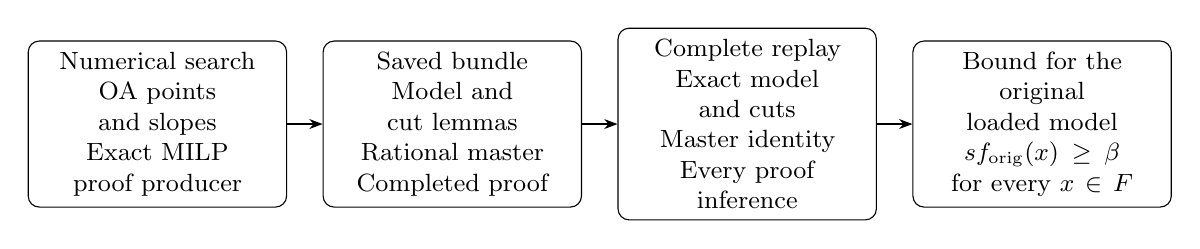
\begin{tikzpicture}[
  box/.style={draw,rounded corners,align=center,text width=3.0cm,
    minimum height=1.8cm,inner sep=4pt,font=\small},
  node distance=0.45cm,>={Stealth}]
\node[box] (search) {Numerical search\\OA points and slopes\\Exact MILP proof producer};
\node[box,right=of search] (bundle) {Saved bundle\\Model and cut lemmas\\Rational master\\Completed proof};
\node[box,right=of bundle] (check) {Complete replay\\Exact model and cuts\\Master identity\\Every proof inference};
\node[box,right=of check] (bound) {Bound for the\\original loaded model\\$s f_{\rm orig}(x)\geq\beta$\\for every $x\in F$};
\draw[->] (search) -- (bundle);
\draw[->] (bundle) -- (check);
\draw[->] (check) -- (bound);
\end{tikzpicture}
\caption{The certificate interface. Complete replay requires every checking obligation to pass; the last implication is objective-preserving bound transfer. Search is outside the trusted base once its output passes. Lean verifies the mathematical contract and typed reference checkers separately, with no verified connection to the Python implementation or benchmark certificates.}
\label{fig:architecture}
\end{figure}

\subsection{Artifact and execution contract}
\label{sec:artifact-contract}
A certificate bundle consists of the supplied model, a nonlinear-lemma file, a rational LP master, and a completed VIPR proof. Each nonlinear lemma names its normalized row and supplies a rational point $z$, a sparse rational slope vector $a$, and an intercept $b$. The checker reconstructs the box and expressions from the model; it does not trust a supplied box, derivative value, curvature label, or reported solver bound. New bundles record the semantic identifier \texttt{pyomo-expression-rationals-v1} and source hash. For compatibility with the saved historical files these fields may be absent; a present identifier must match, and a present source hash is checked. In either case the explicit model passed to replay defines the theorem being checked. The frozen campaign manifest additionally identifies its exact bytes.

Complete checking performs the following operations in order.
\begin{enumerate}
\item Load and validate the model, normalize the objective and nonlinear rows, check domains and curvature, extract exact affine rows, and propagate rational bounds.
\item Reconstruct each lemma's row and symbolic derivatives, verify its point and variable names, and recompute a rigorous intercept bound. Require the supplied $b$ to be no larger than that bound.
\item Regenerate the LP master and require byte equality with the saved LP file. Compare the VIPR problem against the reconstructed rational master semantically, as specified below.
\item Check every supplied master solution and every discrete proof step. Require a finite minimization lower bound for the normalized master. If an external checker was requested, require matching successful corroboration as well.
\end{enumerate}
Only then does the public routine return \texttt{ok=True} and a bound in the original objective sense. Partial mode returns \texttt{status="partial"}, potentially with \texttt{partial\_ok=True}, but \texttt{ok=False} and no certified bound. A missing proof, exception, unsupported input, or failed check cannot expose a certified numerical result. The lower-level VIPR kernel supports infeasibility and either objective sense; the MINLP interface deliberately supports finite normalized lower-bound reports. Theorems about infeasibility in Section~\ref{sec:soundness} do not enlarge this API.

The model loader executes a Python/Pyomo file and applies a documented dedenting repair to top-level model assignments in converted files. It therefore belongs to trusted input construction. Replay requires one active objective and refuses active disjunctive, logical, or special ordered set (SOS) constraints. Supported source variable and affine-row names follow the identifier pattern of a letter or underscore followed by letters, digits, or underscores; reserved auxiliary names cannot alias original variables. The exact extractor replaces fixed variables by their exact values and performs polynomial coefficient accumulation with rational arithmetic. Nonpolynomial subtrees remain available for original-domain checks, even when multiplied by zero. Differentiation and interval evaluation use the same rational-leaf interpretation, rather than a separate floating-point coefficient aggregation.

\subsection{Sufficient curvature and domain rules}
\label{sec:curvature-rules}
Curvature checking combines composition rules in the spirit of disciplined convex programming \citep{grant2006-dcp} with a small number of algebraic recognizers. Each expression carries a curvature classification and, where justified, rational lower and upper range bounds. These are separate facts: a product may be nonnegative without being convex or concave. Unknown curvature or a missing range endpoint is not replaced by a guessed value.

For completeness, the composition principle is immediate from Jensen's inequality. If $v$ is convex and $u$ is convex and nondecreasing on the range of $v$, apply monotonicity to $v(\lambda x+(1-\lambda)y)\leq\lambda v(x)+(1-\lambda)v(y)$ and then convexity of $u$. If $u$ is convex and nonincreasing, use a concave $v$ instead. Reversing both convexity inequalities gives the corresponding concave rules. The implementation applies these principles to sums, rational scalings, affine absolute values, and the functions in Table~\ref{tab:composition}. Negative scaling interchanges convex and concave classifications.

\begin{table}[htbp]
\centering\small
\caption{Principal scalar composition tests. ``Positive'' means a strictly positive certified lower bound; all original expression domains must also pass.}
\label{tab:composition}
\begin{tabular}{p{0.19\linewidth}p{0.55\linewidth}p{0.14\linewidth}}
\toprule
Expression & Sufficient condition & Curvature\\
\midrule
$\exp(v)$ & $v$ affine or convex & Convex\\
$\log(v)$ & $v$ positive, affine or concave & Concave\\
$\sqrt v$ & $v$ nonnegative, affine or concave & Concave\\
$v^p$, $p\geq1$ & $v$ nonnegative, affine or convex & Convex\\
$v^p$, $0<p<1$ & $v$ nonnegative, affine or concave & Concave\\
$v^p$, $p<0$ & $v$ positive, affine or concave & Convex\\
$v^{2k}$, $k\in\Z_{>0}$ & $v$ affine, or nonnegative convex, or nonpositive concave & Convex\\
$k_0/v$, $k_0>0$ & $v$ positive, affine or concave & Convex\\
$k_0^v$, $k_0>0$ & $v$ affine; also $v$ convex if $k_0>1$, or concave if $k_0<1$ & Convex\\
\bottomrule
\end{tabular}
\end{table}
The power and reciprocal tests follow from first and second derivatives on the stated intervals; for $k_0^v$ use $\exp(v\log k_0)$. Power one preserves curvature, and power zero is the constant one after checking the original base domain. Nonnegative-domain rules extend to an included zero endpoint only when the expression is defined and continuous there. Convexity recognition at such an endpoint does not establish differentiability there.

\paragraph{Quadratic forms and norms.}
For $q(x)=x^\top Qx+b^\top x+c$ with rational symmetric $Q$, global convexity on $\R^n$ is equivalent to $Q\succeq0$ because $\nabla^2q=2Q$. This gives a sufficient test on any certified box, including a box with fixed coordinates. Off-diagonal monomial coefficients are split equally between $Q_{ij}$ and $Q_{ji}$. The exact elimination test uses the following elementary characterization.
\begin{lemma}[Exact quadratic tests]
\label{lem:quadratic-recognition}
For symmetric $Q$, a positive leading pivot $\alpha$ in
$Q=\left[\begin{smallmatrix}\alpha&v^\top\\v&C\end{smallmatrix}\right]$
reduces positive semidefiniteness to $C-vv^\top/\alpha\succeq0$. A negative diagonal entry rules it out. A zero diagonal entry requires its whole remaining row and column to be zero, in which case they can be removed. These rules give an exact rational test. Moreover, if
\[
 H=\begin{bmatrix}Q&b/2\\b^\top/2&c\end{bmatrix}\succeq0,
\]
then $\sqrt{q(x)}$ is globally defined and convex.
\end{lemma}
\begin{proof}
For $\alpha>0$, completing the square writes the quadratic form as
$\alpha(t+v^\top z/\alpha)^2+z^\top(C-vv^\top/\alpha)z$.
A negative diagonal gives a negative value on a coordinate vector. If a diagonal is zero and some corresponding entry $v_j$ is nonzero, the restriction to those two coordinates has a term $2v_jt$ with no $t^2$ term and takes negative values. This proves the elimination rules by induction. For the second statement, factor the real positive semidefinite matrix as $H=R^\top R$. Then $\sqrt{q(x)}=\|R(x,1)\|_2$, the norm of an affine map, and the triangle inequality proves convexity. The factor need not be rational or computed by the checker; exact testing of $H$ is sufficient.
\end{proof}
Testing $-Q$ gives concavity. The homogenized test is used only as a sufficient recognition rule for square roots of quadratics; no claim is made to recognize every convex square-root expression. At a norm origin, finite subgradients may exist even though the symbolic-gradient route abstains.

\paragraph{Monomials and geometric means.}
The algebraic recognizer collects rational exponents in
$m(x)=\prod_i x_i^{\alpha_i}$ on a positive orthant. It accepts convexity when all $\alpha_i\leq0$, or when exactly one exponent is positive and $\sum_i\alpha_i\geq1$. It accepts concavity when all $\alpha_i\geq0$ and $\sum_i\alpha_i\leq1$. A rational coefficient scales or reverses the result. These established conditions are stated by \citet[Theorems~2.1--2.2, p.~507]{lundell2009-signomial}, who attribute them to earlier work. We include a direct proof to make the recognition contract self-contained and avoid reliance on floating eigenvalue calculations.
\begin{lemma}[Monomial tests]
\label{lem:monomial-recognition}
The preceding sufficient curvature tests hold on the positive orthant. When all nonzero exponents are positive, the resulting convexity or concavity extends continuously to the nonnegative orthant wherever the product is so defined.
\end{lemma}
\begin{proof}
With $D=\operatorname{diag}(1/x_i)$, differentiation gives
\[
 \nabla^2m(x)=m(x)D\bigl(\alpha\alpha^\top-\operatorname{diag}\alpha\bigr)D.
\]
If every $\alpha_i\leq0$, the middle matrix is the sum of a positive semidefinite outer product and a nonnegative diagonal matrix. For nonnegative exponents, weighted Cauchy--Schwarz yields
$(\sum_i\alpha_i u_i)^2\leq(\sum_i\alpha_i)\sum_i\alpha_i u_i^2$,
so the middle matrix is negative semidefinite if the exponent sum is at most one.

For the remaining convex case remove zero exponents and write $\alpha=(p,-b_1,\ldots,-b_k)$ with $b_i>0$, $B=\sum_i b_i$, and $p\geq1+B$. The lower block of the middle matrix is $\operatorname{diag}(b)+bb^\top\succ0$, and
$b^\top(\operatorname{diag}(b)+bb^\top)^{-1}b=B/(1+B)$,
as follows by multiplying that matrix by $\mathbf 1/(1+B)$. Its Schur complement is $p(p-1)-p^2B/(1+B)=p(p-1-B)/(1+B)\geq0$. If $k=0$, this is simply $p(p-1)\geq0$. The Hessian criteria prove the interior assertions. Taking limits of the convexity inequalities proves their continuous boundary extensions.
\end{proof}
The syntax recognizer restricts fractional powers of products to justified nonnegative variable factors and a unit constant before distributing the exponents. Original denominator and power domains are checked first. Thus it does not use identities such as $\sqrt{x^2}=x$ on a negative domain. For example, the product-range calculation can prove $xy\geq0$ for $x,y\geq0$, after which the exponent test recognizes the concavity of $\sqrt{xy}$. It never labels the bilinear product itself concave for that reason.

\paragraph{One-variable linear fractions.}
A further rule recognizes $(\alpha x+\beta)/(\gamma x+\delta)$ when the denominator is bounded strictly away from zero with a constant sign. For $\gamma\ne0$, write
\[
 \frac{\alpha x+\beta}{\gamma x+\delta}
 =\frac{\alpha}{\gamma}+\frac{k}{\gamma x+\delta},\qquad
 k=\beta-\frac{\alpha\delta}{\gamma}.
\]
Its second derivative is $2k\gamma^2/(\gamma x+\delta)^3$. Convexity therefore holds when $k$ and the denominator have the same sign, concavity when their signs differ, and the function is constant if $k=0$. A constant denominator uses rational scaling instead. This is a one-variable test; it is not a general curvature test for ratios or perspectives. The former perspective shortcut was disabled because curvature of the inner expression on its own variable bounds need not justify curvature on the actual ratio domain.

\paragraph{Domain and range enforcement.}
Range propagation uses rational endpoint arithmetic for sums, scales, integer powers, and finite products. Finite products use all four endpoint products. On sign-certified half-lines the corresponding extreme products give the finite endpoint, and unsupported sign combinations return an unknown range. Exponential, logarithmic, and rational-power endpoint bounds use outward interval arithmetic at 128-bit precision, with exact rational extraction of their dyadic endpoints. Precision affects how often a strict sign can be proved, not the logical sign criterion.

The original tree is visited before simplification. Division and negative integer powers require the relevant range to exclude zero strictly; logarithms require positivity. Noninteger constant powers require a nonnegative base for positive exponents and a positive base for negative exponents. Variable powers require a positive base. A square root requires nonnegativity, possibly supplied by Lemma~\ref{lem:quadratic-recognition}. Only the stated arithmetic nodes and supported unary functions are admitted. These checks take place on declared bounds, not on a domain inferred from nonlinear constraints. A model can therefore be mathematically convex and feasible yet be rejected by the sufficient rules.

\subsection{Interval cut replay and numerical proposals}
\label{sec:cut-implementation}
The nonlinear expression is translated to SymPy with exact rational leaves, and symbolic derivatives are built from that same expression. The interval evaluator implements addition, multiplication, powers, exponential, logarithm, and absolute value. A rational point is converted by interval division of its integer numerator and denominator, never through a binary64 approximation. Rational powers are evaluated with the applicable square-root or exponential/logarithm formula. If a formula or derivative is unsupported, undefined, or nonfinite at the point, the cut is refused. In particular, recognizing an absolute value or norm as convex does not provide a general nonsmooth derivative rule.

The precise bridge from differentiation to \eqref{eq:g-support} is a derivative along feasible segments, not merely a list of finite coordinate differences. If, for each $x\in B$, the right derivative of $\theta\mapsto g(z+\theta(x-z))$ at zero is $p^\top(x-z)$, convexity gives
\[
 g(x)-g(z)\geq \lim_{\theta\downarrow0}
 \frac{g(z+\theta(x-z))-g(z)}{\theta}=p^\top(x-z).
\]
A differentiable extension near $z$ is sufficient; valid relative-domain chain rules can also give this condition at a boundary. The symbolic-expression layer is trusted to provide derivatives with this meaning. Finiteness of arbitrary one-sided coordinate derivatives alone would not suffice: $-\sqrt{xy}$ on the nonnegative quadrant has zero derivatives along the two axes at the origin, but the zero vector does not support it. The implemented symbolic quotient derivatives are singular there and the cut is rejected. Likewise, singular derivatives of $-\sqrt{x}$ and unsupported sign expressions at norm origins are refused. Removable singularities can be simplified only consistently with the original checked domain. These are explicit obligations of the expression and differentiation implementation, not consequences of interval finiteness or a mechanized verification of every accepted expression.

Cut checking uses a 200-bit interval context. All function and derivative endpoints must be finite. The right-hand side of \eqref{eq:safe-intercept} is enclosed by interval operations, including the maximum of its two endpoint products on a finite coordinate. The final endpoint's sign, integer mantissa, and binary exponent are read directly and converted to a rational. This avoids rounding the endpoint through a different precision before comparing it to the supplied intercept. The arithmetic libraries and symbolic derivative implementation remain trusted components of this operation.

The numerical producer uses a separate loaded model. Its OA log supplies candidate row names, points, and slopes; exact reconstructed rows define the certificate mathematics. Points are rationalized and clipped to the propagated box. Slopes are initially shortened to 12 significant decimal digits by default, with directed repairs on one-sided coordinates and exact slopes where available on free coordinates. The intercept is rounded downward to 30 significant decimal digits after rigorous evaluation. These digit counts control representation and practical replay robustness; they provide no universal separation margin between two independent interval evaluations. Complete replay still requires the exact inequality $b\leq$ the newly computed lower endpoint, with no tolerance. Poor points or broad enclosures can lead to fewer cuts or weaker bounds.

\subsection{Binding the discrete proof to the master}
\label{sec:master-identity}
The LP writer includes rational affine rows, accepted cut rows, explicit finite bounds, integrality declarations, and the normalized objective. Every free variable has explicit infinite bounds. Fixed variables retain equal bounds, and a nonzero affine objective constant is carried by a new variable \texttt{objconst} fixed to one. This prevents a silent loss of the constant during proof export. An epigraph coordinate is real and free. Integer bounds tightened by propagation are justified by Lemma~\ref{lem:propagation}.

The VIPR problem parser is shared with the proof kernel. Comparison requires the same variable set under a bijection, the same integer-variable set, minimization sense, and identical rational objective coefficients. A uniform single \texttt{t\_} prefix introduced by SCIP can be removed only if this yields that bijection; genuine original names with that prefix are preserved when already matched. Constraints and bounds are compared as multisets after dividing each nonzero row by the absolute value of its first coefficient in sorted variable order. This permits positive rational row scaling, retaining the relation direction. The current matcher is deliberately stricter than general linear equivalence: it does not recognize arbitrary equivalent row transformations or negative scaling even of equalities. Additional, missing, or altered rows are rejected. A certificate for a different presolved model cannot pass merely because it has the same reported optimum.

The saved LP must also equal the regenerated LP byte for byte. This adds an artifact consistency check; the semantic VIPR comparison supplies the mathematical link to the proof. Original zero-coefficient affine tautologies are omitted in both constructions, and contradictory constant rows are rejected earlier. A hash or LP byte comparison alone cannot replace proof-input matching.

\subsection{Proof grammar, arithmetic, and streaming}
\label{sec:proof-implementation}
The kernel accepts complete proofs in a restricted subset of VIPR versions 1.0 and 1.1. It requires the section order
\[
 \texttt{VER, VAR, INT, OBJ, CON, RTP, SOL, DER}
\]
with the declared numbers of variables, indices, rows, solutions, and derivations. Input uses ASCII integer or fraction tokens with positive denominators; decimal and exponent notation are outside this parser's contract. Variable names, integer indices, vector coefficient indices, and linear-combination references must satisfy the corresponding uniqueness and range checks, including entries whose value is zero. Omitted solution coordinates mean zero and are still checked against all original rows and integrality conditions. The finite primal endpoint of a range report requires a feasible solution attaining that endpoint or a better one.

Each noncomment derivation occupies one line and carries a complete \texttt{asm}, \texttt{sol}, \texttt{lin}, \texttt{rnd}, or \texttt{uns} reason implementing Proposition~\ref{prop:vipr-invariant}. Row labels are metadata; references identify rows by indices. The \texttt{OBJ} coefficient abbreviation denotes the exact parsed objective. Arithmetic uses rational numbers through python-flint. A combination with incompatible inequality directions or a stronger-than-justified right-hand side is rejected even if its discrepancy is numerically small. Assumptions arise only from actual assumption rows and are tracked through every nonzero inference term.

The checker requires every inference reference to precede its row, including references with zero multipliers. A lifetime annotation is $-1$ or a nonnegative in-range index; references after a stated last use are errors. The optional single terminal \texttt{global} marker emitted by SCIP is accepted only if the independently computed assumption set is empty. It cannot remove assumptions or validate a coefficient. Repeated markers, incomplete reasons, unexpected extra tokens, missing derivations, and noncomment suffix material beyond the declared count are rejected.

An assumption-free row dominating the requested dual endpoint or contradiction is recorded as the proving derivation. It need not be the final row. Every declared later derivation must still pass, and the parser must consume the entire file. Consequently a valid proof prefix followed by invalid arithmetic cannot be accepted. A later valid but weaker bound is harmless. The lower-level kernel can also accept a range with no finite dual endpoint when its remaining obligations hold; the MINLP interface requires a finite lower endpoint before reporting a result.

Large proofs are processed in two passes. A first pass validates record shapes, references, and lifetime annotations and computes actual last uses with two arrays of eight-byte integers, about 16 bytes per row. A second pass retains one such array and live sparse rows, freeing a row only after its computed final reference. Rows annotated $-1$ are therefore also freed when safe. The parser initially holds the original master rows for solution checking; this storage and the longest input line must be included in memory accounting. The method avoids storing the whole proof text, but has no constant-memory guarantee: many simultaneously live dense rows, long rational tokens, or a large original master can still consume substantial memory.

\subsection{Failures that motivated the checking boundary}
\label{sec:checker-repairs}
Two small counterexamples show why an external success message is insufficient. The inspected upstream \texttt{viprchk} checkout\footnote{VIPR checkout \texttt{30f2951d1e90e47afa821bdd1b12b82246656c42}; the audit records the source hash and regression inputs. The statement concerns those inspected bytes.} used an initially zero best objective for a solution inference even with an empty solution section. A matching artifact for $\min x$ subject to $x\geq1$ could thereby receive acceptance for a claimed lower bound of $10^6$, although $x=1$ is feasible. The new kernel refuses a solution cutoff without an exactly checked witness. Wood et al.\ also discuss solution-inference and reference-management weaknesses in older checker behavior \citep{wood2026-vipr-smt}; this work makes no priority claim for identifying that general risk.

The second reproduced defect rounded the continuous inequality $x\geq1/2$ to $x\geq1$. This implication is false, even when every printed coefficient is rational. The corrected rule checks both integer coefficients and integer variable declarations before applying a floor or ceiling. Likewise, complementary branch inequalities form an exhaustive disjunction only for an integral linear form. Merely seeing adjacent integer right-hand sides is insufficient.

Other targeted regressions cover exact floating-leaf aggregation, lost domains after cancellation, singular norm derivatives, omitted slopes on half-lines and free coordinates, objective constants and maximization signs, source/master mismatches, invalid solution witnesses, cross-branch assumption retention, duplicate entries, invalid lifetimes, forged \texttt{global} markers, and invalid suffixes after an already sufficient bound. These tests establish distinct observable contracts; passing them is not a formal proof of the parser or executable.

The distinction between rejection and refutation is material. An insufficient safe-cut enclosure can reject a globally valid cut. An unsupported curvature rule can reject a convex model. In contrast, an exact arithmetic audit can establish that a particular recorded inference is invalid. Even the latter does not prove the final bound false if some different valid proof exists. The experimental section therefore retains these outcomes separately rather than relaxing the check to recover historical success labels.

\subsection{Generation, frozen replay, and trust}
\label{sec:trust}
The current producer uses numerical OA with Gurobi and IPOPT, followed by exact SCIP and VIPR completion tools. It first tries its default exact-SCIP configuration and can retry with selected separation, presolve, and propagation features disabled. Each attempt has its own search budget, and proof completion and checking add time. A solver time limit is consequently not a total pipeline wall-clock limit. Fraction canonicalization in newly generated completed proofs preserves their rational values; solution sections and inference meanings are not rewritten to obtain acceptance. Existing historical artifact directories are preserved.

Replay requires only the checker dependencies: Pyomo, NumPy, SymPy, mpmath, and python-flint, together with the included Python modules. Neither Gurobi, IPOPT, nor SCIP is required to check an already complete bundle. The optional external \texttt{viprchk} must return a zero status and one complete range message matching the exact internal result; it is additional corroboration. The generation harness requests this corroboration, while standalone replay need not.

The campaign wrapper hashes model, lemma, LP, and proof files before and after checking. It records source and environment identifiers, input records, optional external-checker identity, explicit missing/rejected/verified/error/timeout outcomes, and the original record index. Resume requires matching artifact fingerprints and the inputs, source/environment identifiers, external checker, and timeout pinned in the manifest; worker parallelism may change. A worker runs in its own process group so its timeout also stops descendant checkers. Completed output records are flushed; only an interrupted final JSON fragment may be recovered. These measures provide provenance and detect ordinary changes; they do not establish semantic equivalence or protect against an adversary that changes and restores a file during verification. Stable artifact contents and trusted model execution remain explicit execution assumptions. Summaries report whether all expected record indices are present exactly once and use exact rational objective-sense comparisons before converting values for display. An incomplete cohort can still be summarized, with its completeness flag false.

The trusted computing base comprises the loader and exact reconstruction, domain/range and curvature rules, symbolic differentiation, interval arithmetic and endpoint conversion, rational propagation, serialization and master comparison, proof parser and rational kernel, their libraries, and the runtime. The numerical search and proof producer need not be trusted when their outputs pass this contract. Shared trusted code can create common failures, so separate replay and adversarial tests reduce dependence on the numerical solver without eliminating implementation trust. Focused proof-assistant theorems in the following section address only their stated mathematical coverage; they do not automatically certify this entire software stack or every benchmark artifact.

\section{Proof-assistant verification of the mathematical contract}
\label{sec:formalization}
The certificate interface has a standalone formalization in Lean~4 \citep{demoura2021-lean4}. Its coverage inventory lists 49 mathematical obligations from Sections~\ref{sec:model}--\ref{sec:implementation}: propagation, supporting cuts, curvature rules, discrete inference, master identity, bound transfer, and the stated mathematical examples. A claim-to-theorem map gives the precise hypotheses and declarations for each obligation. The formalization verifies the mathematical contract and includes executable Lean checkers for typed discrete proofs and rational quadratic matrices. It does not establish that the Python implementation refines those checkers, and no benchmark certificate is checked by Lean.

\subsection{Nonlinear cuts and recognition rules}
The coordinate type distinguishes bounded intervals, both half-lines, and the real line, so infinite endpoints never enter real arithmetic. The proofs establish the exact suprema in Table~\ref{tab:shift}, including attainment and the necessary and sufficient finiteness conditions, as well as the enclosure tests in Table~\ref{tab:enclosure}. Rational propagation instructions preserve every mixed-integer feasible point through any finite admitted sequence, including integer rounding, binary intersections, and fixed substitution. Convexity and a justified derivative along each feasible segment imply the supporting inequality. The cut theorem combines that support with genuine value and residual-slope enclosures and the rational intercept test to derive affine underestimation on the whole box. Interval lemmas prove the finite endpoint arithmetic and the sign-dependent rules for unbounded coordinates; they do not verify the execution of an interval library.

The curvature proofs cover the stated composition rules with their domain and sign conditions, quadratic convexity and concavity, PSD homogenization and square-root convexity, real-exponent monomials, and one-variable linear fractions. Quadratic elimination is a structurally recursive rational checker with soundness and completeness proofs for symmetric matrices, including singular and zero-pivot cases. The monomial development proves the actual second derivative in every direction and its displayed Hessian matrix expression, the three exponent criteria, the supporting block identities, and the continuous boundary extensions. These results concern the mathematical functions and checked domains; recognizing their syntax in a loaded expression is a separate implementation obligation.

\subsection{Discrete checking and end-to-end transfer}
The Lean discrete checker consumes rational rows with equality or either weak inequality, declared integer coordinates, rational solution candidates, and a finite list of typed inference steps. It checks row domination, multiplier signs, integral rounding, and exhaustive integer splits. References address only the checked prefix, assumption sets retain their exact indices, and unsplitting removes each branch's own assumption without erasing cross-branch dependencies. The theorem \texttt{Discrete.check\_sound} proves the complete inference invariant from these tests. Every supplied row is checked, including rows after an earlier proving row. Rational solution validation and a proved finite-minimum selection supply the weak incumbent cutoff; \texttt{Discrete.checked\_bound} then proves the unrestricted master bound. Maximization follows by objective negation, and the separate infeasibility checker uses no solution cutoff.

The end-to-end development constructs the feasible extension rather than assuming its inclusion in the master. It connects admitted propagation steps, accepted supporting-cut data, original affine rows, and integrality to the graph point with its free epigraph coordinate and fixed-one constant coordinate. The affine and epigraph objectives preserve the normalized original objective exactly. A typed master-identity check proves equivalence under variable renaming, integrality correspondence, positive rational row scaling, and complete row permutations, together with objective equality. The resulting bound theorems compose those results with the discrete checker; the sign and infeasibility corollaries have the interpretations stated in Section~\ref{sec:bound-transfer}.

Primal completion uses an actual feasible nonlinear witness and an objective enclosure. The proofs establish nonemptiness and boundedness before applying the real infimum, derive the bound chain and gap, and prove attainment when the bounds match. Separate extended-real results cover the empty feasible set. The formal examples also check the coefficient-aggregation arithmetic, the complete slope-rounding calculation, boundary-support cautions, invalid inference examples, and domain counterexamples. Kernel-evaluated discrete examples exercise accepted splitting and rounding, rejected forward references and later invalid rows, retained cross-branch dependencies, and rejected infeasible or fractional incumbents.

\subsection{Validation and trust boundary}
The package pins Lean~4.33.1 and mathlib~4.33.1 \citep{mathlib2020}, with exact transitive revisions in its manifest. The current development was checked with targeted module builds that treat warnings as failures; we report no result of the project-wide verification script. That script checks complete module imports, builds the project, audits every owned declaration for transitive axioms, and replays compiled declarations through the installed Lean kernel. Its axiom allowlist is \texttt{propext}, \texttt{Classical.choice}, and \texttt{Quot.sound}; the replay is another pass through the same kernel, with imported mathlib as the dependency base. An earlier replay of three modules is kept as a historical record and does not cover the current development.

The remaining trust boundary is operational. Python model loading, expression extraction, symbolic differentiation, actual interval enclosures and transcendental evaluation, serialization, VIPR text parsing, mutable row storage, lifetime accounting, and correspondence between Python execution and the typed Lean checkers are not formally verified. Nor do the proofs verify saved benchmark bundles, external-checker behavior, performance measurements, or novelty claims. The recognition rules are sufficient, not complete for all convex expressions or all valid cuts. Accepted nonlinear evidence must still supply genuine derivative and enclosure data for the same interpreted model.

\section{Computational evidence and independent solution audits}
\label{sec:experiments}

The results establish three practical properties of the interface. First,
a frozen uniform experiment yields accepted bound artifacts for 203 of 289
attempted models in separate replay, with 80 accepted bounds satisfying $0\le d\le10^{-2}$ for the signed
normalized reference difference defined below.
Those references are unverified, so proximity does not establish optimality.
Second, exact audits distinguish invalid supplied proof steps and infeasible
returned points from failures of sufficient nonlinear checks. Third, saved
proofs make checking independent of repeating numerical search, but their
storage and replay costs remain substantial. We examine capability, failure
mechanisms, and costs in that order. Appendix~\ref{app:experimental-accounting}
retains the complete protocol, production accounting, and separately versioned
repair results; none of those later checks replaces the frozen uniform outcome.

\subsection{Capability: checkable bounds and their strength}
\label{sec:replay-results}

The frozen repository catalogue contains 299 models selected for convexity and
discrete variables from MINLPLib~\citep{minlplib}. Seven selected files did not
load and three did not pass the then-used curvature screen. The remaining 289
names form the complete denominator of the historical and uniform campaigns. The supplement
lists all 299 names and the ten exclusions, including their recorded reasons.
The selection is a repository snapshot, not a claim about the current size or
classification of MINLPLib. We distribute the loaded Python model files with
MINLPLib's CC-BY~4.0 attribution. GAMS is the library's primary representation;
the certificates concern the exact loaded expression semantics of
Section~\ref{sec:model}, not an unverified equivalence of every converted model.

The uniform protocol gives numerical OA and each exact-SCIP attempt a
requested 30-second search budget, allows at most a default and a conservative
fallback attempt, and caps each complete instance process group at 360 seconds.
It uses six workers, followed by a separate execution of the same checker with
six workers and a 1,200-second per-record limit. The search budgets exclude
additional preprocessing, proof completion, and checking work covered by the
outer cap. All 289 names remain in the denominator, including failed generation.

Separate replay accepts 203 artifacts, rejects 19, and finds 67 without a
complete bundle (Table~\ref{tab:campaign-results}). The producer itself returns
198 accepted results. Four additional accepted artifacts survive outer
timeouts and one survives a worker error. Thus an unsuccessful process return
need not destroy a completed checkable proof. This distinction measures the
availability of justified bounds under the stated protocol, rather than only
the producer's return status. It does not establish coverage of all convex
MINLPs or superiority over another solver.

\begin{table}[tb]
\centering
\caption{Complete replay outcomes and exact reference comparisons. Both denominators are 289; generation outcomes are reported separately in the text. Historical replay also used external corroboration. Reference rows count only verified bounds; $d$ is the signed normalized difference from an unverified reference (Section~\ref{sec:reference-comparison}).}
\label{tab:campaign-results}
\begin{tabular}{lrr}
\toprule
Quantity & Historical archive & Uniform-run artifacts \\
\midrule
Verified & 188 & 203 \\
Near reference: $0\le d\le10^{-4}$ & 52 & 46 \\
Near reference: $0\le d\le10^{-2}$ & 81 & 80 \\
Negative reference difference & 23 & 25 \\
Rejected & 92 & 19 \\
Missing complete artifacts & 9 & 67 \\
Timed out during replay & 0 & 0 \\
Other replay errors & 0 & 0 \\
\bottomrule
\end{tabular}
\end{table}


\paragraph{Strength relative to recorded objectives.}
\label{sec:reference-comparison}
For a replayed bound $B$ in the original objective sense, a recorded library
objective $r$, and $s=1$ for minimization or $s=-1$ for maximization, we compute
\[
        d(B,r)=\frac{s(r-B)}{\max\{1,|r|\}}.
\]
The bound and the decimal reference string are converted to exact rationals
before subtraction. We report the number satisfying $0\le d\le 10^{-4}$ and
$0\le d\le 10^{-2}$, and report $d<0$ separately. This is a signed normalized
difference from an unverified reference, not an optimality gap. Even $d=0$
does not prove that a feasible nonlinear point exists at that value.

Among the 203 accepted uniform-run bounds, 46 satisfy the first threshold
and 80 the second; 25 differences are negative. The interface therefore
produces some bounds close to recorded objectives, while the uniform success
count alone does not imply tight bounds. Among the 188 accepted historical
bounds, 52 satisfy the first threshold and 81 satisfy the second. The
historical comparison has 23 negative differences; every magnitude is
below $6\cdot10^{-10}$. Such small differences can arise from rounded reference
strings. In particular, we do not convert their sign into a claim of an
incorrect solver result. The supplement records every exact comparison,
including the uniform campaign's results in Table~\ref{tab:campaign-results}.
\paragraph{Bounds versus completed optimality proofs.}
A close reference value supplies no primal witness. Exact original-model
feasibility checks do complete the bound for \texttt{clay0204m}, giving optimum
6545 (Section~\ref{sec:solver-audits}), and for the small quadratic example
below. These are positive examples of the stronger conclusion available when
the primal and bound evidence match; we do not infer a benchmark optimality
count from objective comparisons.

The core's solver-free replay includes a mixed-integer quadratic example,
$\min y$ subject to $(x-\tfrac12)^2\le y$, $x\in\{0,1\}$ and $0\le y\le2$.
Eleven checked cuts and 39 proof derivations establish the lower bound
$1/4$, attained by $(x,y)=(0,1/4)$. The \texttt{clay0204m} matching-point audit
and the targeted repaired examples exercise larger complete bundles. These
checks supplement the 161 targeted software tests; test counts are not a
formal proof of the implementation. Section~\ref{sec:formalization} specifies
the separate proof-assistant result and its boundary.

Beyond the uniform experiment, the retained historical and targeted repair
artifacts form a useful descriptive collection. The repair versions and their
separate denominators are specified in Appendix~\ref{app:repair-accounting}.
The descriptive merged catalogue contains verified bounds for 222 distinct loaded models. It chooses the strongest exact normalized lower bound among 405 accepted records from the historical, primary, producer-repair, and reporting-repair evidence, requiring identical model SHA-256 and objective sense for every comparison. Exact ties use a fixed cohort order. Each entry identifies its original-sense bound, complete proof, source cohort, and hashes. This union is a reusable bound collection; its coverage is not attributed to the uniform search budget.


\subsection{Failure mechanisms: what rejection establishes}
\label{sec:failure-mechanisms}

A rejection is informative only when tied to its checking obligation. The
uniform run's 67 admission errors occur at the curvature/domain check, before
master generation; they account for all 67 missing replay bundles. Its nineteen
rejections comprise eighteen proof-rule or proof-grammar failures and one
post-proof reporting failure. The latter concerns representation of an already
checked exact bound, not failure of its mathematical inferences. Separately
recorded repairs address that boundary and twelve producer normalization
failures without changing the proof, domain, curvature, propagation, or
master-matching rules (Appendix~\ref{app:repair-accounting}).

\paragraph{Invalid supplied discrete inferences.}
Three new completed proofs receive an external acceptance message but fail
local conditions of the internal rules. Two linear combinations mix opposite
inequality directions: in each, a strictly positive multiplier of an upper
branch row appears among lower-row terms. The offending rows have nonzero
coefficients and are not constant tautologies. In the third proof, an
\texttt{uns} step cites the same integer coordinate $u$ with branches
$u\le64$ and $u\ge66$. Integer activity 65 is uncovered. Other master rows might
in principle exclude that activity, but the submitted standalone disjunction
step does not establish such an exclusion. The supplement gives the exact
antecedents and multipliers. These observations concern the individual supplied
inferences and do not imply false final bounds.

These cases show why external acceptance does not discharge the internal
inference obligations. The exact row directions and uncovered integer activity
supply local witnesses that are stronger evidence than process status or a
small objective discrepancy.

The historical audit provides a broader check on the effect of enforcing all
layers of the contract. Of 269 historical records labeled accepted, 188
retain that verdict. The 81
revocations comprise 67 domain or curvature failures, 13 cut-verification
failures, and one discrete-proof failure. Eleven further discrete-proof
failures came from historical records already labeled as crashed, giving 92
current rejections in total. Nine records lack a completed proof. No record in
the complete historical replay timed out or mutated during checking.
These counts replace the historical acceptance claim; the archived old flags
are retained solely to make the change auditable.

The twelve historical failures that reach the discrete proof checker admit
small exact arithmetic audits. In eleven, the claimed upper row has exactly
the coefficients obtained by the supplied rational linear combination, but
its right-hand side is smaller than that combination permits. The exact
positive excess ranges from approximately $1.55\cdot10^{-12}$ to
$1.93\cdot10^{-10}$. An arbitrarily small excess still invalidates that
inference over the reals. In the remaining instance,
\texttt{smallinvDAXr5b200-220}, a positive multiplier uses an upper inequality
in a combination requiring lower inequalities; the multiplied directions are
incompatible. The portable supplement includes the twelve first-failure
steps, their referenced rows, and an independent \texttt{Fraction}-arithmetic
recombination script. Full completed proofs are in the bulk archive.
These are invalid justifications, not proofs that their final proposed bounds
are unattainable or false.

\paragraph{Conservative nonlinear failures.}
Nonlinear rejection has a different interpretation. For example, the first
historical \texttt{risk2bpb} cut exceeds the newly recomputed sufficient safe
intercept by approximately $1.17\cdot10^{-12}$. This establishes failure of
this certificate test, not global invalidity of the affine inequality.
A separately recorded repaired generation for \texttt{risk2bpb} passes all
checks and gives an original-sense bound of approximately $-55.876139395$.
The library string $-55.8761394$ lies slightly beyond this bound; the difference
is consistent with rounding at the reference's displayed precision. Targeted repaired generations for
\texttt{batchdes}, \texttt{clay0204m}, and \texttt{risk2bpb} are retained as
regression evidence, separate from the uniform campaign.

This distinction is essential to interpreting the rejection counts: an exact
invalid inference refutes its submitted justification, whereas a failed
sufficient enclosure or curvature test may reflect the limits of the admitted
certificate rather than a false inequality or a nonconvex model.

\paragraph{Returned points and matching primal evidence.}
\label{sec:solver-audits}
Objective disagreements guide investigation; original-variable checks determine
what can be concluded about a returned point. For saved solver objectives
$r_{\rm solver}$, we include recorded GAMS model
statuses 1 (Optimal), 2 (Locally Optimal), and 8 (Integer Solution),\footnote{GAMS 53 User's Guide, \href{https://www.gams.com/53/docs/UG_GAMSOutput.html}{Model Status table}.}
and flag pairs satisfying
\[
 s(B-r_{\rm solver})>10^{-6}\max\{1,|B|\}.
\]
This one-sided criterion flags 18 historical bound/solver pairs. These are investigation candidates;
the two returned-point audits below support stronger, explicitly limited
conclusions.

For \texttt{clay0204m}, a saved SBB run reports objective 5075 with normal
completion and model status \emph{Integer Solution}; its log also warns of a
nonconvex model. We therefore do not describe it as an unqualified global
optimality status. Its printed point violates the two rows
\[
 x_2-x_4+51b_{13}\le46.5,\qquad
 x_6-x_7+86b_{24}\le82
\]
by 4.5 and 3, respectively. Allowing every printed coordinate an error of
$0.00005$ changes the row values by at most $0.00265$ and $0.0044$.
The violations are consequently robust to the displayed precision.
Independently, exact rational evaluation of a 52-variable point checks all
90 loaded constraints and 32 binary variables at objective 6545. A complete
certificate proves the matching lower bound 6545. Together these establish
an exact optimum for the loaded model. The archived point comes from rounded
BARON output with small distance coordinates explicitly replaced by zero;
its feasibility follows from the new rational evaluation, not from BARON's
status or tolerance.

For \texttt{risk2bpb}, the saved SHOT run reports an objective near
$-56.82087261$ and optimal model status. Its printed point assigns one to both
$b_4$ and $b_5$, although both variables are fixed at zero in the source model.
These unit violations suffice to reject that returned point. They do not
identify the internal cause of the discrepancy. The archived run used SHOT
1.1 with CPLEX 22.1; the baseline scripts requested 60 seconds, relative and
absolute optimality tolerances $10^{-4}$ and $10^{-6}$, and four threads.

To ensure that these statements compare the intended formulas, a separate
source audit matches the GAMS and loaded Python models under the same exact
binary64-constant interpretation. It eliminates the GAMS free objective
variable and defining equality, then compares each remaining constraint,
variable type, fixed value, and bound with an explicit index map. The
\texttt{clay0204m} comparison maps 53 variables and 91 rows to 52 variables
and 90 rows; \texttt{risk2bpb} maps 464 variables and 581 rows to 463 variables
and 580 rows. The audited violated rows and fixed bounds use exactly
representable coefficients, so their violations do not depend on a distinction
between decimal and binary64 constants. This is source-formula equivalence;
it does not verify the GAMS compiler or recover either solver's historical
in-memory model. The conclusions concern the saved returned points and the
specified source models, without attributing an unobserved internal defect.

The point audits establish concrete feasibility failures, and the separate
\texttt{clay0204m} witness establishes exact optimality for the loaded model.
Neither conclusion relies on treating a solver status or library objective as
a primal certificate. The source comparison states precisely which model is
being checked, while leaving the compiler and unseen solver state outside the
claim.

\subsection{Costs and practical limits}
\label{sec:experimental-costs}

Replay avoids repeating numerical search, but does not make large certificates
cheap to store or check. The uniform campaign takes 2,840.697 seconds of elapsed
generation time; its later separate replay takes 533.541 seconds. Accepted
checker calls sum to 2,791.064 seconds, with median 5.173 and maximum 221.484;
all 289 records sum to 2,953.982 seconds. These are observed shared-machine
costs with concurrent workers, not serial elapsed times or controlled speed
comparisons. Complete checking includes nonlinear/model checks, master matching,
and proof replay, rather than only discrete inference arithmetic. Historical
replay additionally includes external corroboration; its full costs are kept
separate in Appendix~\ref{app:experimental-accounting}.

The 203 accepted uniform proofs occupy 14,233,742,052 bytes and contain
11,749,855 derivations. The accepted historical proofs occupy
38,826,726,525 bytes; their median size is 74,469,242 bytes and their largest
is 2,163,285,624 bytes. Retaining failed completed proofs and fallback attempts
adds further audit value and storage cost. The complete proof collection is
30,664,561,063 bytes compressed and contains 93,713,729,595 regular-file bytes;
a small core supports representative replay without extracting that collection
(Appendix~\ref{app:reproduction}). These observations establish a practical
storage burden, not a certificate-size comparison with prior methods.

The machine provides approximately 30\,GiB of memory and 18 physical cores
(36 logical processors). Six instance workers share those resources. OA,
SCIP, and LP search request one thread each; proof completion retains its tool
defaults, so the entire pipeline is not single-threaded. The two-pass replay
in Section~\ref{sec:implementation} avoids retaining the whole proof text and
frees sparse rows after their last use. Its storage still includes per-derivation index arrays and depends on the
original master, input-line length, rational sizes, and simultaneously live
rows; machine capacity is not a measurement or bound on checker peak memory.
We infer no memory or speed advantage from these runs. The complete hardware,
software, timeout, phase-accounting, and hashing protocol is retained in
Appendix~\ref{app:experimental-accounting}.

A small portable core contains the checker sources, pinned dependency
specifications, all 289 campaign models, compact campaign records and exact comparison
tables, the source and returned-point audit, and representative certificates.
The separate bulk archive contains the completed historical and new proofs,
including rejected completed attempts. Generator dependencies are documented
separately: running the checker does not require Gurobi, IPOPT, SCIP, or GAMS.
License-identifying solver banners are removed only from distributed log
copies; the redaction manifest records original and distributed hashes.
Model files, mathematical data, and proof files are unmodified.

The practical result is a replayable collection with explicit limits: useful
bounds are available for many attempted models, exact audits can localize
specific failures, and expensive saved proofs remain separable from a small
checker-only starting point. The evidence supports those claims without
turning reference proximity, conservative rejection, or shared-machine timing
into stronger conclusions.

\section{Discussion and conclusions}
\label{sec:discussion}
The certificate interface makes the implication from a rational master bound to a convex MINLP bound explicit and checkable. Its essential connection is objective-preserving feasible-set inclusion: rigorously justified cuts retain every nonlinear feasible point, master identity binds those cuts to the discrete proof, and complete rational replay establishes the transferred bound. This allows numerical search to propose evidence without making its tolerances part of the final mathematical assertion.

A first lesson is that exactness must refer to one model throughout the calculation. Exact arithmetic in the discrete proof is insufficient if curvature analysis, derivative evaluation, or master construction interpret an expression differently. The loaded-tree contract fixes the coefficients and domains to which the certificate refers. The bound therefore concerns that exact model; relating it to an earlier modeling file is a further semantic obligation.

A second lesson is that verification failures need mathematical classification. The audits identify invalid supplied linear combinations and integer disjunctions, including steps that received external acceptance. Tiny residuals and successful process status do not justify those steps. Other rejected artifacts fail sufficient domain, curvature, or cut-enclosure tests and may still represent convex models or valid cuts. A local invalid inference refutes its supplied justification, not necessarily its final proposed bound. Retaining the evidence makes these distinctions reproducible.

A third lesson is that primal feasibility supplies information that objective comparisons cannot. Original-variable audits expose violations in two saved solver points, while independently checked original-model witnesses complete exact optimality proofs in two cases. These conclusions require bounds, integrality, rows, and objective evaluation for the same model. A feasible master point or a close library reference value cannot substitute for that work.

The uniform experiment yields accepted artifacts for 203 of 289 attempted models in separate replay, compared with 198 successful producer returns under the stated protocol. Complete proofs surviving unsuccessful producer returns further show the value of separating an artifact's validity from a process outcome. The long-rational failures show that exact values must survive text conversion and reporting as well as inference arithmetic. These results establish capability and identify failure mechanisms; the incomplete admission rules, large proof files, and shared-machine timings limit broader coverage and efficiency conclusions. Two-pass replay reduces the proof rows retained in memory without bounding the number of simultaneously live rows, and the present measurements do not establish a speed advantage over other certificate methods or solvers.

The validation has complementary roles. Executable tests and exact local audits exercise concrete checking behavior; Lean verifies the mathematical contract and the soundness of typed reference checkers for discrete proofs and rational quadratic matrices. These proofs do not verify the model loader, symbolic and interval software, or the Python master matcher and VIPR checker, nor establish their correspondence to the Lean definitions. The completed result is consequently a replayable certificate method for the stated model class with an explicit trust boundary, supported by reproducible capability and reliability evidence.

\appendix
\section{Data, code, and reproduction}
\label{app:reproduction}
The accompanying materials suffice for reading the paper, building its PDF, checking the Lean development, and replaying the reported experimental evidence. They consist of three separate archives; no public deposit or DOI is claimed. The small core and bulk proof archives are identified by byte counts and SHA-256 hashes in \texttt{supplement/archives.json}, which is included with the paper source. MINLPLib inputs retain their attribution and license notice. Installed third-party packages, licensed solver binaries, and user-supplied literature PDFs are not redistributed.

\paragraph{Paper and formal sources.}
The archive \texttt{certified-minlp-paper-source.tar.gz} contains \texttt{main.tex}, all required sections and generated tables, the selected bibliography, the vector figure source, and the standalone \texttt{formal/} project with its dependency pins, coverage statement, and audit scripts. Extract it and run, from the extracted paper directory,
\begin{verbatim}
latexmk -pdf -interaction=nonstopmode -halt-on-error main.tex
\end{verbatim}
A TeX installation with BibTeX and the packages listed in \texttt{main.tex}, including TikZ, is sufficient; no experimental archive is needed. The source archive contains no stale LaTeX auxiliary files or Lean caches. To check the Lean development, install Elan, Git, and Python 3 and run from \texttt{formal/}:
\begin{verbatim}
sha256sum -c verification/extension-SHA256SUMS
lake exe cache get
bash scripts/verify.sh
\end{verbatim}
The toolchain and manifest select the exact Lean and mathlib versions. Downloading the dependency cache is separate from building and replaying the project proofs. The saved three-module replay, which audited 95 declarations, covers only the earlier scope; the current development has separately recorded targeted module checks, and no result of the full script is reported here. Section~\ref{sec:formalization} and the coverage map specify the current mathematical scope and its implementation boundary.

\paragraph{Checker-only core.}
The archive \texttt{certified-minlp-core.tar.gz} is 6,478,681 bytes compressed. It contains all 289 campaign model files, current checker code, pinned dependency specifications, versioned source snapshots, compact records and audit data, representative complete bundles, and the scripts used to regenerate tables and the bound catalogue. Extract it to obtain \texttt{minlp-certified-evidence/}. From that directory, using Python 3.13:
\begin{verbatim}
python3 -m venv replay-env
replay-env/bin/python -m pip install -r requirements-checker.txt
replay-env/bin/python reproduce.py verify
replay-env/bin/python reproduce.py small --out ../small-checks
replay-env/bin/python reproduce.py summaries --out ../summary.json
\end{verbatim}
The five checker dependencies are Pyomo, NumPy, SymPy, mpmath, and python-flint. The \texttt{small} command checks four complete bundles, the exact original-model source and primal audits, and fifteen local failed-step extracts. The 161-test suite additionally needs pytest, as specified in \texttt{requirements-tests.txt}. None of these commands needs licensed optimization software. The core README gives commands that regenerate all thirteen table and catalogue outputs from saved records; this reproduces recorded results, not new solver timings.

\paragraph{Complete proof collection.}
The separate archive \texttt{certified-minlp-certificates.tar.gz} is 30,664,561,063 bytes compressed and contains 93,713,729,595 bytes of regular-file contents. It retains accepted and rejected completed proofs and completed fallback attempts. For full replay, extract it into the same parent directory as the core. The core provides a streaming archive verifier and commands for complete historical and uniform replay and for the separate repair cohorts. A full readback matched all 5,207 archive entries to their recorded file hashes or symlink targets; routine example checking does not require repeating it.

The default distributed checker is version V3; Appendix~\ref{app:repair-accounting} gives the measured V1 outcome and the expected V3 outcome. The core documents restoration of V1, V2, and V3 into separate copies, including shared test and example data. Their restored test counts are 152, 153, and 161, respectively. New replay commands write new records and manifests.

\paragraph{Generation and provenance.}
Appendix~\ref{app:experimental-accounting} specifies the frozen experimental protocols, full production accounting, and separate repair cohorts. Generating new evidence requires the numerical solvers and proof-production tools described in the core README: Gurobi, IPOPT, exact SCIP, and VIPR completion and checking utilities. The wrapper accepts local executable paths and freezes models, software, settings, budgets, and environment before launch. Absolute paths in frozen manifests document the recorded machine; portable replay resolves files relative to the extracted layout. Numerical generation and elapsed times can change with machine load or software builds; exact strings, input hashes, versioned code, and complete outcome records define the reproducible checking claim.

\section{Experimental protocol and supporting accounting}
\label{app:experimental-accounting}

Section~\ref{sec:experiments} organizes the findings by capability, failure
mechanism, and cost. This appendix records the frozen protocols and full
production and repair accounting that support those findings. Its summaries
are derived from the frozen campaign records, with separate denominators for
the primary and targeted runs.

\subsection{Frozen protocols and measurement boundaries}

The historical campaign used a 60-second numerical outer-approximation budget,
heterogeneous exact-SCIP budgets of 180 or 90 seconds, and varying concurrency.
Its archived producer labels are therefore neither current acceptance evidence
nor results of a uniform timing experiment. We replayed all 289 records with
six workers and a 1,200-second per-record limit, including both the internal
exact proof kernel and the external \texttt{viprchk} corroboration. The replay
manifest identifies the checker sources and inputs by SHA-256; the harness
checks artifact hashes again after checking.

We also generated new artifacts for the same 289 names, including every
historical failure, using a protocol frozen before the first run. Numerical
outer approximation and each exact-SCIP attempt received a requested search
budget of 30 seconds. The producer tried its default configuration and, after
an unsuccessful complete check, at most one conservative fallback. We requested
one solver and LP thread and ran six workers. A separate 360-second wall-clock
limit killed the entire instance process group, retaining partial files and
recording the timeout without retry. The 30-second settings are search budgets:
loading, preprocessing, nonlinear subproblem overruns, proof completion, and
checking are additional work covered by the outer limit. Tool events distinguish
SCIP invocations, proof completion, external checking, and internal proof replay.

After generation, a separate complete replay used six workers and a
1,200-second per-record limit. Its acceptance criterion uses a separate
execution of the same internal checker, which is implemented separately from the solver and external VIPR
checker; the generator's external-check results remain additional evidence.
The replay chooses the canonical completed proof when present, otherwise the
completed failed fallback, otherwise the completed failed default attempt.
This rule was fixed before replay and uses no bound-quality selection.
Consequently, a complete proof surviving a producer timeout can earn a
separate replay verdict without being counted as completed production.
All attempt outcomes remain in the data. We rehash the frozen sources, settings,
model inputs, wrapper, and tool executables after generation.

The machine has an Intel Xeon w5-2565X processor (18 physical cores, 36 logical
processors) and approximately 30\,GiB of memory, running Linux under WSL2.
Generation uses Gurobi 13.0.3, IPOPT 3.14.20, and SCIP 10.0.3 with
SoPlex 8.0.3. Package versions, executable hashes, and the full hardware
description are recorded with the protocol. The one-thread setting concerns
OA, SCIP, and LP search; proof completion retains its tool defaults (its
banner reports 36 available threads), so the entire pipeline is not claimed
to be single-threaded. Times are observed costs on a shared machine,
not isolated solver speed comparisons. In particular, sums over concurrent
workers are not campaign elapsed times. Large archive compression takes place
after the timed campaigns.

\subsection{Complete production and replay accounting}

The following generated summary retains every primary V1 production outcome,
including process failures whose surviving artifacts later verify. It also
records the selected proof sizes, derivation counts, and checker timings.
The uniform generation records 198 completed accepted productions, 67 producer errors, 8 unsuccessful completed-check attempts, 4 outer timeouts, and 12 worker errors. Its elapsed time is 2,840.697 seconds. Separate replay accepts 203 bounds, rejects 19 bundles, and finds 67 incomplete bundles. Of its accepted bounds, 4 come from outer-timed-out production, 1 from worker errors, and 0 from producer rejections; 0 use a retained failed-attempt completed proof. Accepted proofs occupy 14,233,742,052 bytes and contain 11,749,855 derivations. Their summed and median checking costs are 2,791.064 and 5.173 seconds, respectively; the maximum is 221.484 seconds. All-record checking costs sum to 2,953.982 seconds and separate replay elapsed time is 533.541 seconds. These observations characterize this fixed protocol, including its unsuccessful attempts; they do not estimate asymptotic coverage or establish superiority over another solver.


All 67 producer errors arise at domain/curvature admission, before master
generation. The nineteen primary replay rejections comprise eighteen proof-rule
or proof-grammar failures and one post-proof rational-reporting failure.
Table~\ref{tab:generation-phases} separates recorded tool phases during
generation; interrupted calls have no imputed completion time.
\begin{table}[tb]
\centering
\caption{Observed in-generation calls in the uniform campaign. Sums include completed calls only; starts without ends are interrupted observations. SCIP times cover the process invocation, not just search. These rows are separate from full pipeline and later replay times.}
\label{tab:generation-phases}
\begin{tabular}{lrrr}
\toprule
Phase & Started & Ended & Seconds (sum) \\
\midrule
SCIP process & 358 & 358 & 7,401.357 \\
Proof completion & 358 & 358 & 371.307 \\
External proof check & 477 & 477 & 1,290.663 \\
Internal proof replay & 202 & 201 & 1,583.153 \\
\bottomrule
\end{tabular}
\end{table}


Under the historical replay protocol, the accepted proofs contain 29,903,993 derivations and occupy
38,826,726,525 bytes. Their median size is 74,469,242 bytes and their largest
size is 2,163,285,624 bytes. Median accepted checking time is 16.679 seconds,
with a maximum of 463.845 seconds. The sum over accepted records is
7,987.954 seconds; the sum over all 289 records is 8,234.349 seconds.
The campaign elapsed time is 1,465.381 seconds. These checking times include
model and lemma validation, master reconstruction, and internal and external
proof checking; the harness records hashing separately. Thus the aggregate
is not a measurement of just the linear-proof kernel.

\subsection{Separately versioned representation repairs}
\label{app:repair-accounting}

V1 denotes the frozen primary producer and checker. V2 repairs producer proof
normalization, and V3 additionally repairs exact rational report input/output.
These changes concern the survival of exact values through textual interfaces,
not additional mathematical proof rules. Keeping all three versions separates
the uniform protocol result from targeted recovery of affected artifacts.

The uniform run exposed twelve worker failures when proof normalization passed
a rational token through Python's decimal-to-integer conversion limit. We
preserved this campaign and its producer source, then replaced that conversion
with parsing and serialization through the existing FLINT rational type.
A separate cohort regenerated all twelve observed occurrences under the same
requested search budgets, settings, concurrency, and outer limit. The original
289-record denominator and its failures remain unchanged.

A further reporting boundary appeared in \texttt{tls12}: its primary bundle
passed nonlinear checks, exact master matching, and the entire proof kernel,
but a rational bound with a 4,326-digit numerator failed during subsequent
report construction. The same
boundary appeared in the default attempt of the producer-repair cohort.
A third source version repairs exact rational text input and output at the
reporting interfaces, including replay comparisons and reference summaries.
Decimal reference strings retain exact decimal semantics; the interpreter's
global integer-conversion guard remains enabled. Optional binary64 display
values become unavailable when the exact value is outside binary64 range,
while exact strings remain authoritative. The proof, domain, curvature,
propagation, and master-matching rules are unchanged.

All twelve producer-repair runs returned verified output, and all twelve
selected bundles passed separate replay. Generation took 478.703 seconds of
elapsed time and replay took 62.473 seconds. Auditing all nineteen primary
rejections and all secondary attempt reports identified exactly two completed
proofs affected by the subsequent reporting defect, both for \texttt{tls12}.
With the third source version, both passed full replay in a separate
73.431-second cohort, without further optimization. The frozen primary replay
counts remain 203 verified and 19 rejected; the corrected reporting layer
accepts one additional primary bundle. The supplement preserves the sources,
records, and completed attempts for each version. These targeted repairs do
not constitute a second uniform experiment or replace its denominator.


The current checker is V3. Its two targeted checks establish one additional
accepted primary artifact; they do not constitute a new full 289-record replay.
A complete V3 replay of the fixed primary artifacts is expected to give
204 verified, 18 rejected, and 67 missing, subject to the documented time and
environment limits. The measured uniform outcome remains V1's 203/19/67.
Appendix~\ref{app:reproduction} specifies the version restoration and replay
commands. The descriptive catalogue combines protocols by matching model
hashes and objective senses; its 222-model coverage is not attributed to a
single search budget.

\bibliographystyle{plainnat}
\bibliography{references}
\end{document}
